% Gerado de CSVs agregados; dados numericos incorporados para portabilidade.
% Notebook SHA-256: e8ce396c21be212f5a12d673622adf543234983c3cd142088ea2dbe8e7621004
% Parecer SHA-256: 1ee24339005b98f24afb2375d080f1aaa8ff1ab0e8812427b8b103b890cef98a
% Requer: pgfplots, biblioteca statistics (somente taxas.tex).
% Ajuste opcional no chamador: \def\AlturaGrafico{4.4cm} e \def\LarguraGrafico{\linewidth}.
\begingroup
\providecommand{\AlturaGrafico}{4.4cm}
\providecommand{\LarguraGrafico}{\linewidth}
\definecolor{grafverde}{HTML}{24574D}
\definecolor{grafazul}{HTML}{1769A5}
\definecolor{grafgrafite}{HTML}{253A40}
\definecolor{graflaranja}{HTML}{B97736}
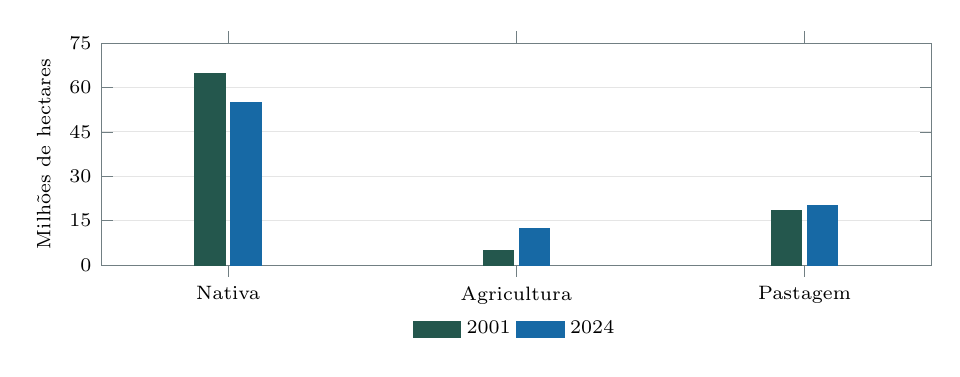
\begin{tikzpicture}
\begin{axis}[width=\LarguraGrafico,height=\AlturaGrafico,
font=\scriptsize,tick label style={font=\scriptsize},
label style={font=\scriptsize},
axis line style={grafgrafite!65},tick style={grafgrafite!65},
grid style={black!10},
legend style={font=\scriptsize,draw=none,fill=none,cells={anchor=west}},
/pgf/number format/use comma,
ybar,bar width=11pt,ymin=0,ymax=75,ytick={0,15,30,45,60,75},
symbolic x coords={Nativa,Agricultura,Pastagem},xtick=data,
enlarge x limits=0.22,ymajorgrids=true,
ylabel={Milh\~oes de hectares},
legend columns=2,legend style={at={(0.5,-0.20)},anchor=north},
]
\addplot+[fill=grafverde,draw=grafverde,area legend] coordinates {(Nativa,64.6733010293) (Agricultura,5.0039899540) (Pastagem,18.3858676477)};
\addplot+[fill=grafazul,draw=grafazul,area legend] coordinates {(Nativa,54.9390637610) (Agricultura,12.4175621478) (Pastagem,20.2049180566)};
\legend{2001,2024}
\end{axis}
\end{tikzpicture}
\endgroup
